% Created 2021-09-11 Sat 08:17
% Intended LaTeX compiler: xelatex
\documentclass[letterpaper]{article}
\usepackage{graphicx}
\usepackage{grffile}
\usepackage{longtable}
\usepackage{wrapfig}
\usepackage{rotating}
\usepackage[normalem]{ulem}
\usepackage{amsmath}
\usepackage{textcomp}
\usepackage{amssymb}
\usepackage{capt-of}
\usepackage{hyperref}
\usepackage[margin=1in]{geometry}
\usepackage{fontspec}
\usepackage{indentfirst}
\setmainfont[ItalicFont = LiberationSans-Italic, BoldFont = LiberationSans-Bold, BoldItalicFont = LiberationSans-BoldItalic]{LiberationSans}
\newfontfamily\NHLight[ItalicFont = LiberationSansNarrow-Italic, BoldFont       = LiberationSansNarrow-Bold, BoldItalicFont = LiberationSansNarrow-BoldItalic]{LiberationSansNarrow}
\newcommand\textrmlf[1]{{\NHLight#1}}
\newcommand\textitlf[1]{{\NHLight\itshape#1}}
\let\textbflf\textrm
\newcommand\textulf[1]{{\NHLight\bfseries#1}}
\newcommand\textuitlf[1]{{\NHLight\bfseries\itshape#1}}
\usepackage{fancyhdr}
\pagestyle{fancy}
\usepackage{titlesec}
\usepackage{titling}
\makeatletter
\lhead{\textbf{\@title}}
\makeatother
\rhead{\textrmlf{Compiled} \today}
\lfoot{\theauthor\ \textbullet \ \textbf{2021-2022}}
\cfoot{}
\rfoot{\textrmlf{Page} \thepage}
\titleformat{\section} {\Large} {\textrmlf{\thesection} {|}} {0.3em} {\textbf}
\titleformat{\subsection} {\large} {\textrmlf{\thesubsection} {|}} {0.2em} {\textbf}
\titleformat{\subsubsection} {\large} {\textrmlf{\thesubsubsection} {|}} {0.1em} {\textbf}
\setlength{\parskip}{0.45em}
\renewcommand\maketitle{}
\author{Houjun Liu}
\date{\today}
\title{Lazer Scanners/Printers}
\hypersetup{
 pdfauthor={Houjun Liu},
 pdftitle={Lazer Scanners/Printers},
 pdfkeywords={},
 pdfsubject={},
 pdfcreator={Emacs 27.2 (Org mode 9.4.4)}, 
 pdflang={English}}
\begin{document}

\maketitle


\section{Lazer Printers + Scanners w.r.t. Electrostatics}
\label{sec:orgf0ae9f3}
\begin{figure}[htbp]
\centering
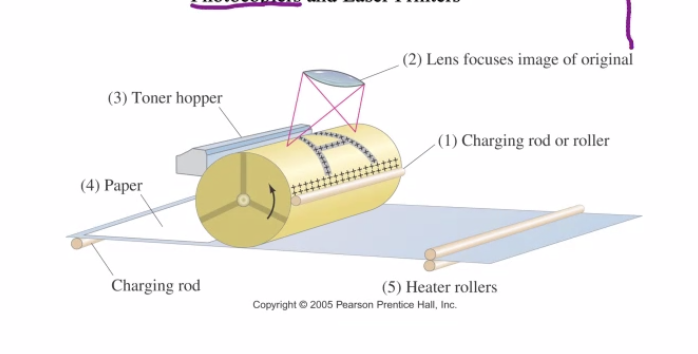
\includegraphics[width=.9\linewidth]{./Screen Shot 2020-09-09 at 10.46.29 AM.png}
\caption{Screen Shot 2020-09-09 at 10.46.29 AM.png}
\end{figure}

\subsection{Lazer scanner\ldots{}}
\label{sec:org3821949}
\begin{enumerate}
\item LED light cause original to reflect into mirror
\item Scanning drum (yellow thing) does electrostatics!

\begin{enumerate}
\item Drum plated with plastic
\item Positively charged drum gets positively charged by a smaller
roller
\item Light reflecting off of the original (the parts of the original
without black ink, anyway) disturbs the positively charged roller
\item Plastic becomes conducting where it experiences light
\item Drum under the positive is \textbf{grounded} --- meaning it could absorb
\begin{itemize}
\item apply an infinite amount of electrons, so any grounded
\end{itemize}
conductor becomes neutral
\item You could see from the figure above, where you have dark on the
original, positive charge contributed by (4) is left on the
plastic. Where you have light, the plastic becomes a conductor
and the ground draws the electrons away, making light parts
neutral
\item Now, the toner powder next to the drum will only stick to the
positive parts of the plastic printing drums, which, remember, is
where light paper\textsubscript{did} not\_ affect
\item And then, a copy!
\end{enumerate}
\end{enumerate}

Lazer printing works in the same way as above, except plastic becomes
conducting where it experiences light from a computer-controlled laser
drawing a negative of the print.
\end{document}
